\documentclass[11pt,a4paper]{article}
\usepackage[margin=18mm,headheight=15pt]{geometry}
\usepackage[T1]{fontenc}
\usepackage[utf8]{inputenc}
\usepackage{lmodern}
\usepackage{microtype}
\usepackage{xcolor}
\usepackage{graphicx}
\usepackage{booktabs}
\usepackage{tabularx}
\usepackage{array}
\usepackage{enumitem}
\usepackage{amsmath}
\usepackage{tikz}
\usetikzlibrary{arrows.meta,positioning,shapes.geometric,shapes.multipart,fit,backgrounds,calc,matrix}
\usepackage[most]{tcolorbox}
\usepackage{fancyhdr}
\usepackage{titlesec}
\usepackage{hyperref}
\usepackage{lastpage}
\usepackage{ragged2e}
\usepackage{multicol}
\usepackage{pdflscape}
\usepackage{float}

\definecolor{navy}{HTML}{12304A}
\definecolor{blue}{HTML}{176B87}
\definecolor{teal}{HTML}{2A9D8F}
\definecolor{mint}{HTML}{DDF3EF}
\definecolor{sky}{HTML}{E6F2F8}
\definecolor{gold}{HTML}{E9A23B}
\definecolor{coral}{HTML}{D96853}
\definecolor{ink}{HTML}{24313A}
\definecolor{muted}{HTML}{60717D}
\definecolor{paper}{HTML}{F7FAFB}
\definecolor{line}{HTML}{B8C7CF}

\hypersetup{colorlinks=true,linkcolor=blue,urlcolor=blue,citecolor=blue,
  pdftitle={AI-Assisted Cancer Diagnosis: Cognitive Computing Design},
  pdfauthor={Cognitive Computing Course Report}}
\color{ink}
\setlength{\parindent}{0pt}
\setlength{\parskip}{5pt}
\setlist{nosep,leftmargin=5mm}
\renewcommand{\arraystretch}{1.24}
\pagestyle{fancy}
\fancyhf{}
\lhead{\small\color{muted}AI-Assisted Cancer Diagnosis}
\rhead{\small\color{muted}Cognitive Computing}
\cfoot{\small\color{muted}\thepage\ of \pageref{LastPage}}
\titleformat{\section}{\Large\bfseries\color{navy}}{\thesection}{0.6em}{}
\titleformat{\subsection}{\large\bfseries\color{blue}}{\thesubsection}{0.55em}{}
\titlespacing*{\section}{0pt}{12pt}{5pt}
\titlespacing*{\subsection}{0pt}{8pt}{3pt}

\tikzset{
  >={Latex[length=2.2mm]},
  flow/.style={->,thick,draw=blue},
  softflow/.style={->,thick,draw=muted,dashed},
  box/.style={rounded corners=2mm,draw=blue,thick,fill=sky,align=center,
    minimum height=10mm,text width=31mm,font=\small},
  tealbox/.style={box,draw=teal,fill=mint},
  goldbox/.style={box,draw=gold,fill=gold!10},
  coralbox/.style={box,draw=coral,fill=coral!10},
  darkbox/.style={box,draw=navy,fill=navy,text=white},
  circlebox/.style={circle,draw=blue,thick,fill=sky,align=center,
    minimum size=18mm,font=\small\bfseries}
}

\newtcolorbox{keybox}[1][]{enhanced,breakable,colback=sky,colframe=blue,
  boxrule=0.7pt,arc=2mm,left=3mm,right=3mm,top=2mm,bottom=2mm,#1}
\newtcolorbox{warningbox}[1][]{enhanced,breakable,colback=gold!8,colframe=gold,
  boxrule=0.7pt,arc=2mm,left=3mm,right=3mm,top=2mm,bottom=2mm,#1}
\newcommand{\badge}[1]{\tikz[baseline=(x.base)]\node[rounded corners=1mm,fill=teal,
  text=white,font=\scriptsize\bfseries,inner xsep=1.5mm,inner ysep=.7mm](x){#1};}

\begin{document}

\begin{titlepage}
\pagecolor{navy}
\color{white}
\vspace*{16mm}
{\small\bfseries\color{teal!60}\MakeUppercase{Cognitive Computing Case Study}\par}
\vspace{10mm}
{\fontsize{29}{34}\selectfont\bfseries AI-Assisted Cancer Diagnosis\par}
\vspace{4mm}
{\Large Human Judgment and Cognitive Systems\par}
\vspace{10mm}
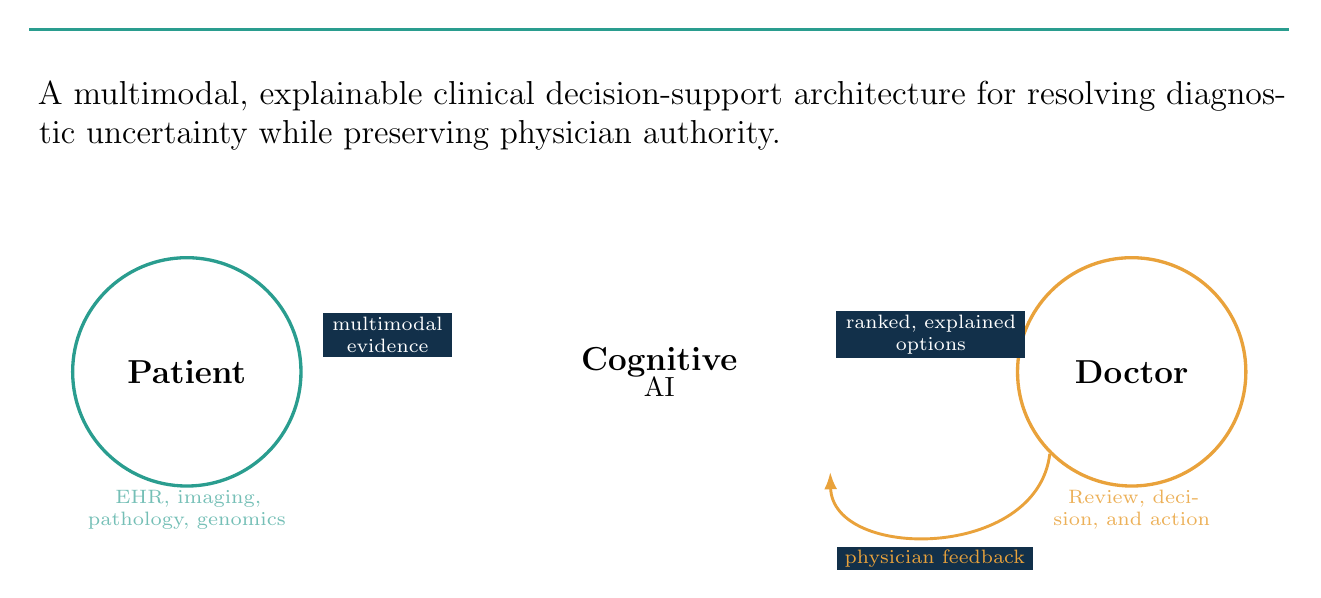
\begin{tikzpicture}[x=1cm,y=1cm]
  \draw[teal,line width=1.2pt] (0,0) -- (16,0);
  \node[anchor=west,text width=15.8cm,align=left,font=\large] at (0,-1.1)
  {A multimodal, explainable clinical decision-support architecture for resolving diagnostic uncertainty while preserving physician authority.};
  \node[circle,draw=teal,line width=1.2pt,minimum size=29mm,align=center] (p) at (2,-4.35)
    {\large\bfseries Patient};
  \node[rounded corners=3mm,draw=white,line width=1.2pt,
    minimum width=43mm,minimum height=25mm,align=center] (ai) at (8,-4.35)
    {\large\bfseries Cognitive\\[-1mm]AI};
  \node[circle,draw=gold,line width=1.2pt,minimum size=29mm,align=center] (d) at (14,-4.35)
    {\large\bfseries Doctor};

  \draw[->,white,line width=1.3pt] (p.east) -- (ai.west);
  \node[fill=navy,inner xsep=1.2mm,inner ysep=.5mm,align=center,
    font=\scriptsize,text=white] at (4.55,-3.88) {multimodal\\evidence};

  \draw[->,white,line width=1.3pt] (ai.east) -- (d.west);
  \node[fill=navy,inner xsep=1.2mm,inner ysep=.5mm,align=center,
    font=\scriptsize,text=white] at (11.45,-3.88) {ranked, explained\\options};

  \node[text width=31mm,align=center,font=\scriptsize,text=teal!65] at (2,-6.1)
    {EHR, imaging, pathology, genomics};
  \node[text width=43mm,align=center,font=\scriptsize,text=white!75] at (8,-6.1)
    {Fusion, probabilistic reasoning, XAI};
  \node[text width=31mm,align=center,font=\scriptsize,text=gold!85] at (14,-6.1)
    {Review, decision, and action};

  \draw[->,gold,line width=1.05pt]
    (d.south west) .. controls (12.8,-6.75) and (10.2,-6.75) .. (ai.south east);
  \node[fill=navy,inner xsep=1mm,inner ysep=.4mm,font=\scriptsize,text=gold]
    at (11.5,-6.72) {physician feedback};
\end{tikzpicture}
\vfill
\begin{tcolorbox}[colback=navy!82!black,colframe=white!30,coltext=white,boxrule=.6pt,arc=2mm]
\textbf{Scenario.} Three oncologists propose Stage II lung cancer, tuberculosis, and a benign pulmonary nodule for the same patient. The design below converts disagreement into an auditable differential diagnosis and a safe plan for confirmatory testing.
\end{tcolorbox}
\vspace{8mm}
{\small Course: Cognitive Computing \hfill Design report and visual architecture\par}
\end{titlepage}
\pagecolor{white}
\color{ink}
\tableofcontents
\newpage

\section{Design Position and Clinical Goal}

The proposed platform is a \textbf{clinical decision-support system (CDSS)}. It augments oncologists by organizing evidence, quantifying uncertainty, retrieving relevant knowledge, and explaining alternatives. It does not replace a physician, independently declare a final diagnosis, or silently retrain itself in production.

\begin{keybox}
\textbf{Core objective:} transform heterogeneous evidence into a ranked differential diagnosis, show why each alternative is plausible or weak, identify the next test with the greatest expected diagnostic value, and preserve a complete human-review trail.
\end{keybox}

\subsection{Design principles}
\begin{multicols}{2}
\begin{itemize}
  \item \textbf{Patient-specific:} combine longitudinal context, not isolated measurements.
  \item \textbf{Multimodal:} jointly interpret text, images, laboratory values, genomics, and time series.
  \item \textbf{Probabilistic:} represent ambiguity instead of forcing a binary answer.
  \item \textbf{Explainable:} expose supporting, opposing, and missing evidence.
  \item \textbf{Human-governed:} require clinician confirmation for consequential actions.
  \item \textbf{Continuously improved, not continuously unstable:} deploy only validated model versions.
\end{itemize}
\end{multicols}

\begin{figure}[H]
\centering
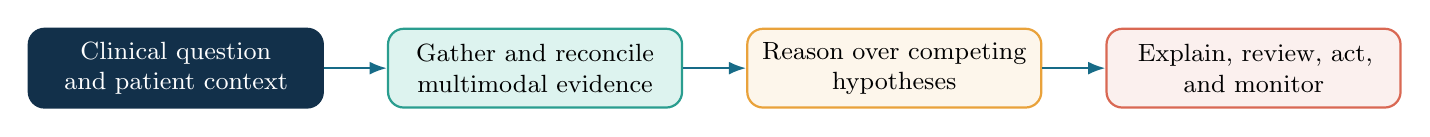
\begin{tikzpicture}[node distance=8mm]
  \node[darkbox,text width=35mm] (q) {Clinical question\\and patient context};
  \node[tealbox,right=of q,text width=35mm] (e) {Gather and reconcile\\multimodal evidence};
  \node[goldbox,right=of e,text width=35mm] (r) {Reason over competing\\hypotheses};
  \node[coralbox,right=of r,text width=35mm] (a) {Explain, review, act,\\and monitor};
  \draw[flow] (q)--(e); \draw[flow] (e)--(r); \draw[flow] (r)--(a);
\end{tikzpicture}
\caption{The system's clinical reasoning contract.}
\end{figure}

\section{Cognitive Computing Architecture}

\subsection{End-to-end architecture}

\begin{figure}[ht]
\centering
\resizebox{\textwidth}{!}{%
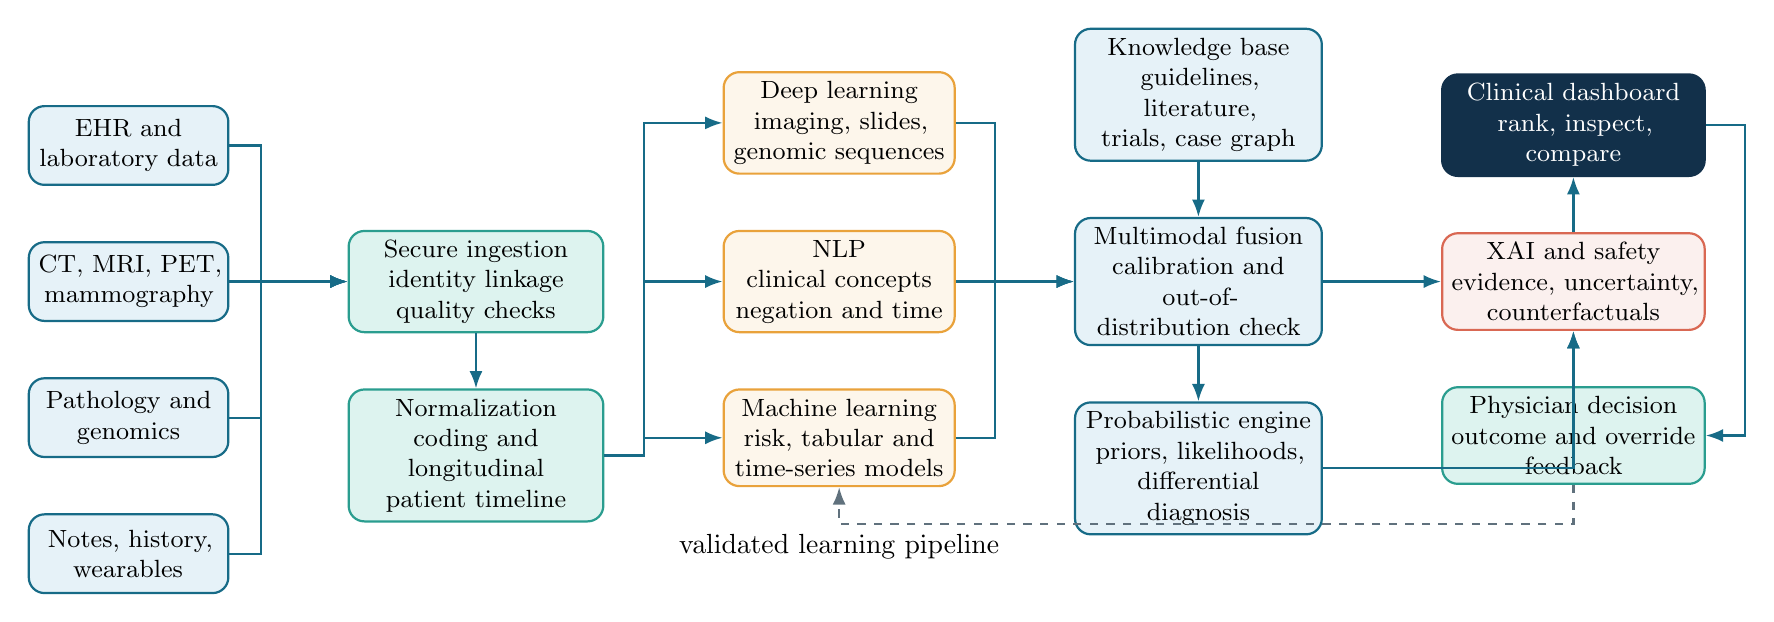
\begin{tikzpicture}[node distance=7mm and 10mm]
  \node[box,text width=23mm] (ehr) {EHR and\\laboratory data};
  \node[box,text width=23mm,below=of ehr] (img) {CT, MRI, PET,\\mammography};
  \node[box,text width=23mm,below=of img] (path) {Pathology and\\genomics};
  \node[box,text width=23mm,below=of path] (text) {Notes, history,\\wearables};

  \node[tealbox,text width=30mm,right=15mm of img] (ingest) {Secure ingestion\\identity linkage\\quality checks};
  \node[tealbox,text width=30mm,below=of ingest] (fhir) {Normalization\\coding and longitudinal\\patient timeline};

  \node[goldbox,text width=27mm,right=15mm of ingest] (nlp) {NLP\\clinical concepts\\negation and time};
  \node[goldbox,text width=27mm,above=of nlp] (dl) {Deep learning\\imaging, slides,\\genomic sequences};
  \node[goldbox,text width=27mm,below=of nlp] (ml) {Machine learning\\risk, tabular and\\time-series models};

  \node[box,text width=29mm,right=15mm of nlp] (fusion) {Multimodal fusion\\calibration and\\out-of-distribution check};
  \node[box,text width=29mm,above=of fusion] (kb) {Knowledge base\\guidelines, literature,\\trials, case graph};
  \node[box,text width=29mm,below=of fusion] (prob) {Probabilistic engine\\priors, likelihoods,\\differential diagnosis};

  \node[coralbox,text width=31mm,right=15mm of fusion] (xai) {XAI and safety\\evidence, uncertainty,\\counterfactuals};
  \node[darkbox,text width=31mm,above=of xai] (ui) {Clinical dashboard\\rank, inspect, compare};
  \node[tealbox,text width=31mm,below=of xai] (feedback) {Physician decision\\outcome and override\\feedback};

  \foreach \s in {ehr,img,path,text} \draw[flow] (\s.east) -- ++(4mm,0) |- (ingest.west);
  \draw[flow] (ingest)--(fhir);
  \foreach \t in {dl,nlp,ml} \draw[flow] (fhir.east) -- ++(5mm,0) |- (\t.west);
  \foreach \t in {dl,nlp,ml} \draw[flow] (\t.east) -- ++(5mm,0) |- (fusion.west);
  \draw[flow] (kb)--(fusion); \draw[flow] (fusion)--(prob);
  \draw[flow] (fusion)--(xai); \draw[flow] (prob.east) -| (xai.south);
  \draw[flow] (xai)--(ui); \draw[flow] (ui.east) -- ++(5mm,0) |- (feedback.east);
  \draw[flow] (feedback)--(xai);
  \draw[softflow] (feedback.south) -- ++(0,-5mm) -| node[below,midway]{validated learning pipeline} (ml.south);
\end{tikzpicture}}
\caption{Reference architecture. Solid arrows represent case-time inference; the dashed arrow represents governed offline improvement.}
\end{figure}

\subsection{Roles of the required cognitive components}

\begin{tabularx}{\textwidth}{>{\bfseries\color{blue}}p{27mm} X X}
\toprule
Component & Primary role & Typical output for this case\\
\midrule
NLP & Convert notes, pathology reports, and literature into structured, contextual clinical concepts; detect negation and temporality. & ``No nodal involvement,'' chronic cough onset, prior TB exposure, lesion descriptors, guideline passages.\\
Machine learning & Model structured clinical and laboratory features; stratify risk; estimate recurrence or response. & Tabular risk scores based on age, smoking, biomarkers, comorbidities, and trends.\\
Deep learning & Analyze images, whole-slide pathology, genomics, and other high-dimensional signals. & Lesion segmentation, margin irregularity, PET uptake pattern, tissue morphology.\\
Knowledge base & Ground reasoning in curated guidelines, staging criteria, drug knowledge, trials, and disease relationships. & Applicable staging rule, differential criteria, guideline version, evidence provenance.\\
Probabilistic reasoning & Combine priors and uncertain evidence; update a differential as evidence changes. & Calibrated probabilities for malignancy, TB, and benign nodule plus uncertainty.\\
Explainable AI & Make model behavior inspectable at patient and model level. & Supporting/opposing evidence, salient image regions, similar cases, counterfactuals.\\
Visualization & Present complexity as a decision workflow rather than a raw model score. & Ranked alternatives, timeline, trends, image overlays, next-test recommendations.\\
\bottomrule
\end{tabularx}

\subsection{Multimodal evidence fusion}

\begin{figure}[ht]
\centering
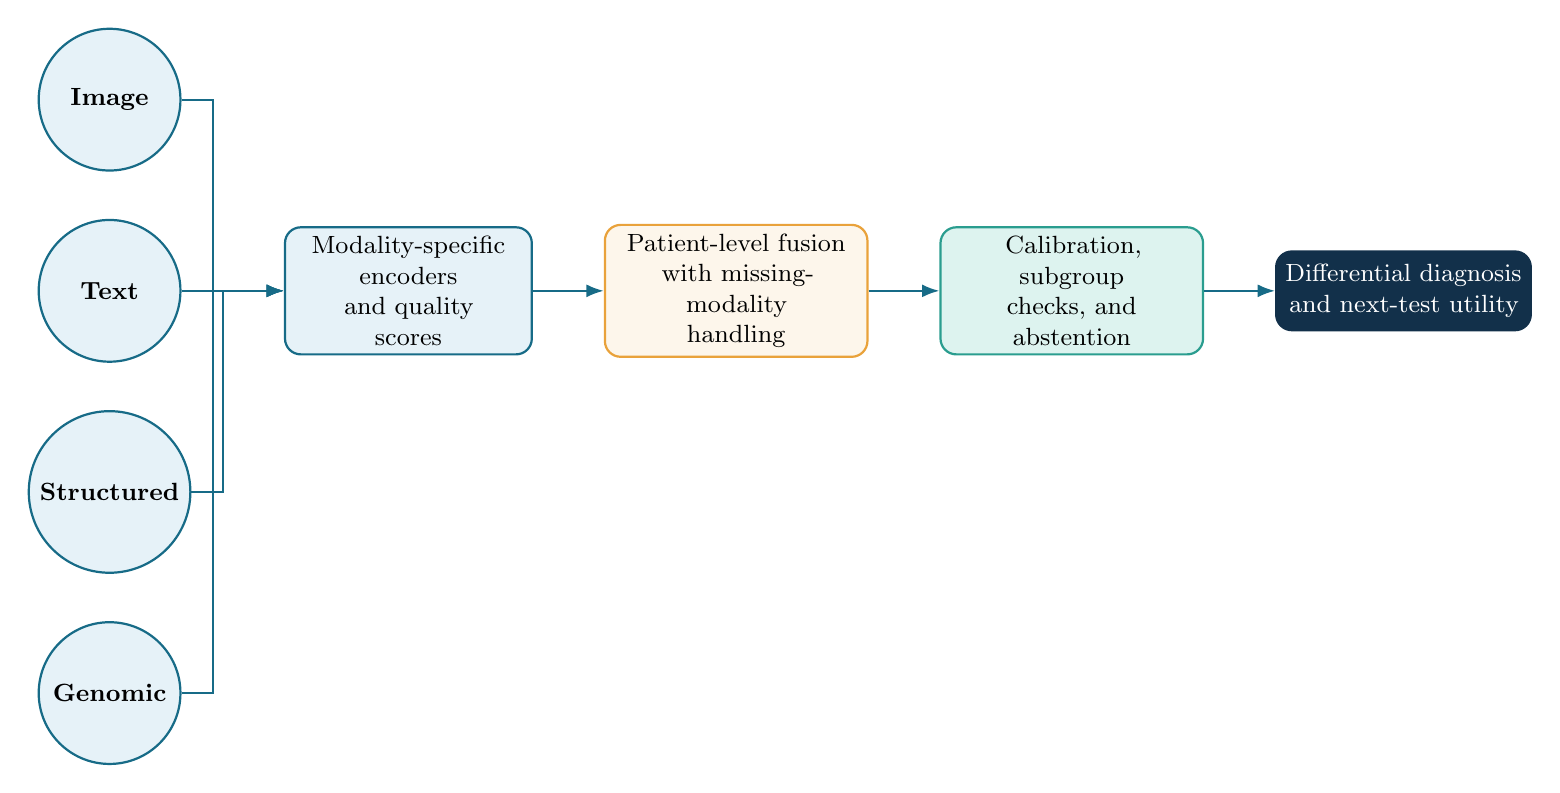
\begin{tikzpicture}[node distance=6mm and 9mm]
  \node[circlebox] (i) {Image};
  \node[circlebox,below=of i] (t) {Text};
  \node[circlebox,below=of t] (s) {Structured};
  \node[circlebox,below=of s] (g) {Genomic};
  \node[box,right=13mm of t,text width=29mm] (enc) {Modality-specific\\encoders and quality\\scores};
  \node[goldbox,right=of enc,text width=31mm] (fuse) {Patient-level fusion\\with missing-modality\\handling};
  \node[tealbox,right=of fuse,text width=31mm] (cal) {Calibration, subgroup\\checks, and abstention};
  \node[darkbox,right=of cal,text width=30mm] (out) {Differential diagnosis\\and next-test utility};
  \foreach \x in {i,t,s,g} \draw[flow] (\x.east) -- ++(4mm,0) |- (enc.west);
  \draw[flow] (enc)--(fuse); \draw[flow] (fuse)--(cal); \draw[flow] (cal)--(out);
\end{tikzpicture}
\caption{Fusion must retain modality quality and missingness, rather than pretending all inputs are equally reliable.}
\end{figure}

\begin{warningbox}
\textbf{Safety boundary.} If required evidence is missing, image quality is inadequate, or the patient lies outside validated populations, the system must lower confidence, explain the limitation, and allow abstention or escalation.
\end{warningbox}

\section{Kahneman's System 1 and System 2}

Kahneman's distinction can be implemented as two cooperating computational modes. It is an analogy for workflow design, not a claim that a model literally thinks like a person.

\begin{figure}[ht]
\centering
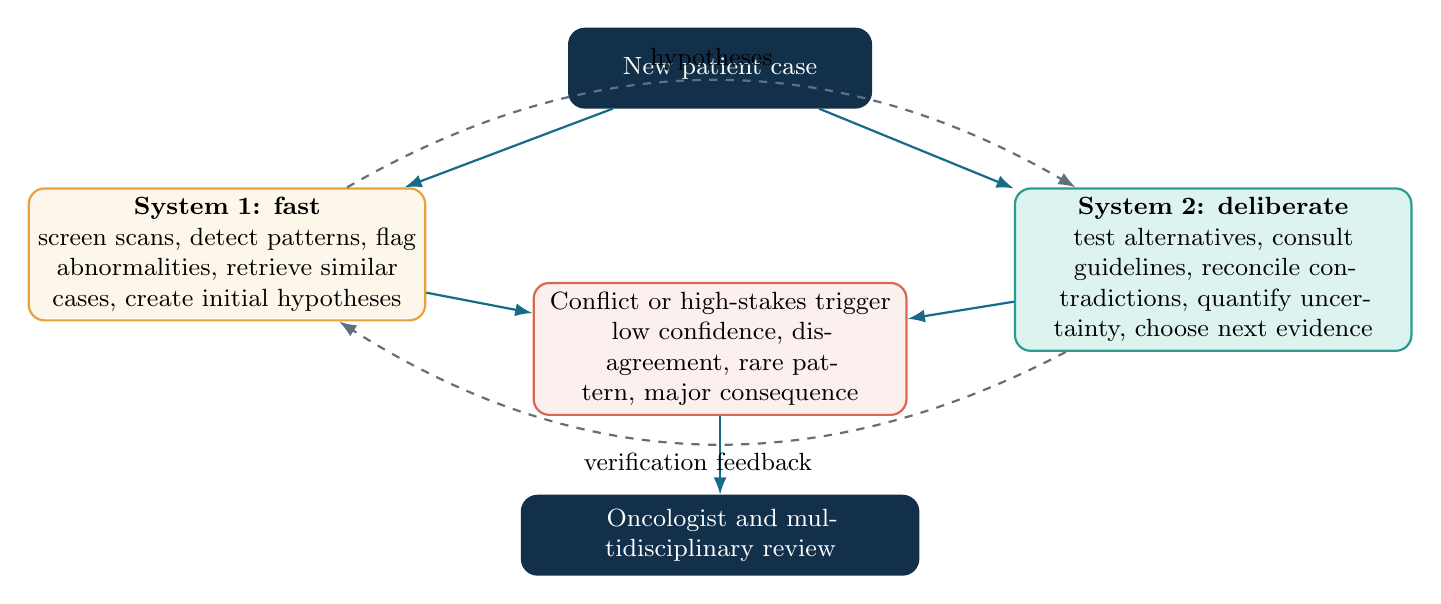
\begin{tikzpicture}[node distance=10mm and 18mm]
  \node[darkbox,text width=36mm] (case) {New patient case};
  \node[goldbox,below left=of case,text width=48mm] (s1) {\textbf{System 1: fast}\\screen scans, detect patterns, flag abnormalities, retrieve similar cases, create initial hypotheses};
  \node[tealbox,below right=of case,text width=48mm] (s2) {\textbf{System 2: deliberate}\\test alternatives, consult guidelines, reconcile contradictions, quantify uncertainty, choose next evidence};
  \node[coralbox,below=22mm of case,text width=45mm] (conflict) {Conflict or high-stakes trigger\\low confidence, disagreement, rare pattern, major consequence};
  \node[darkbox,below=of conflict,text width=48mm] (human) {Oncologist and multidisciplinary review};
  \draw[flow] (case)--(s1); \draw[flow] (case)--(s2);
  \draw[flow] (s1)--(conflict); \draw[flow] (s2)--(conflict);
  \draw[flow] (conflict)--(human);
  \draw[softflow,bend left=30] (s1) to node[above,font=\small]{hypotheses} (s2);
  \draw[softflow,bend left=30] (s2) to node[below,font=\small]{verification feedback} (s1);
\end{tikzpicture}
\caption{Fast recognition proposes; deliberate reasoning challenges; the clinician decides.}
\end{figure}

\subsection{Illustrated collaboration in the disputed lung case}

\begin{enumerate}[label=\textbf{Step \arabic*:},leftmargin=16mm,itemsep=3pt]
  \item \textbf{Rapid screening.} Image and text models detect an irregular pulmonary lesion, weight loss, cough, and inflammatory evidence.
  \item \textbf{Initial hypotheses.} System 1 proposes lung cancer, tuberculosis, and benign pulmonary nodule.
  \item \textbf{Deliberate challenge.} System 2 asks whether infection can mimic the radiologic pattern, checks TB exposure, staging criteria, PET findings, pathology, and data quality.
  \item \textbf{Uncertainty-aware update.} Probabilities are recalibrated and contradictory evidence remains visible.
  \item \textbf{Information-seeking action.} The system recommends biopsy and molecular TB testing because these results are expected to separate the leading hypotheses.
  \item \textbf{Human resolution.} The oncology team reviews evidence, patient preferences, test risks, and timing before deciding.
\end{enumerate}

\begin{figure}[ht]
\centering
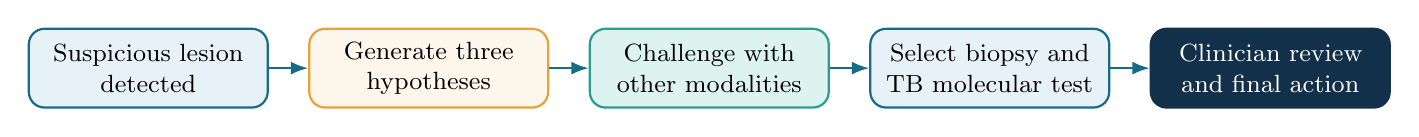
\begin{tikzpicture}[node distance=5mm]
  \node[box,text width=28mm] (detect) {Suspicious lesion\\detected};
  \node[goldbox,right=of detect,text width=28mm] (h) {Generate three\\hypotheses};
  \node[tealbox,right=of h,text width=28mm] (check) {Challenge with\\other modalities};
  \node[box,right=of check,text width=28mm] (test) {Select biopsy and\\TB molecular test};
  \node[darkbox,right=of test,text width=28mm] (review) {Clinician review\\and final action};
  \draw[flow] (detect)--(h); \draw[flow] (h)--(check); \draw[flow] (check)--(test); \draw[flow] (test)--(review);
\end{tikzpicture}
\caption{A practical System 1/System 2 sequence for the case.}
\end{figure}

\section{Rule-Based Expert System vs. Cognitive System}

\begin{tabularx}{\textwidth}{>{\bfseries}p{30mm} X X}
\toprule
Dimension & Traditional rule-based expert system & Proposed cognitive system\\
\midrule
Representation & Fixed IF--THEN rules & Learned models, knowledge graph, probabilistic dependencies\\
Inputs & Mostly manually structured fields & Structured, semi-structured, unstructured, images, genomics, time series\\
Uncertainty & Thresholds and deterministic conclusions & Calibrated distributions, confidence intervals, abstention\\
Adaptation & Experts manually revise rules & Controlled retraining using validated cases and feedback\\
Contradictions & Rule conflicts are brittle to resolve & Weighs conflicting evidence and preserves alternatives\\
Imaging and text & Limited unless manually encoded & Native NLP and deep-learning analysis\\
Output & Often one categorical conclusion & Ranked differential, evidence, uncertainty, and next-test utility\\
Explanation & Trace of fired rules & Local evidence, visual attribution, provenance, counterfactuals, model card\\
Governance & Rule version and author & Data, model, knowledge, calibration, feedback, and override audit trail\\
\bottomrule
\end{tabularx}

\begin{figure}[ht]
\centering
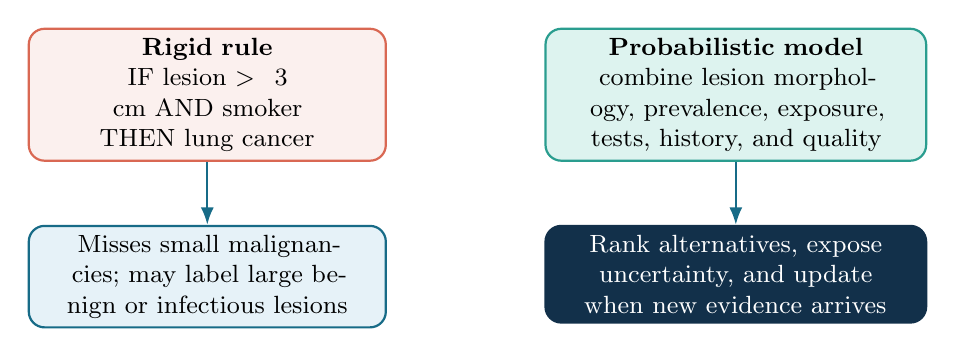
\begin{tikzpicture}[node distance=8mm and 20mm]
  \node[coralbox,text width=43mm] (rule) {\textbf{Rigid rule}\\IF lesion $>3$ cm AND smoker\\THEN lung cancer};
  \node[box,below=of rule,text width=43mm] (fail) {Misses small malignancies; may label large benign or infectious lesions};
  \draw[flow] (rule)--(fail);
  \node[tealbox,right=of rule,text width=46mm] (prob) {\textbf{Probabilistic model}\\combine lesion morphology, prevalence, exposure, tests, history, and quality};
  \node[darkbox,below=of prob,text width=46mm] (rank) {Rank alternatives, expose uncertainty, and update when new evidence arrives};
  \draw[flow] (prob)--(rank);
\end{tikzpicture}
\caption{Deterministic thresholding versus evidence-weighted reasoning.}
\end{figure}

\subsection{Why probabilistic reasoning is appropriate}

Symptoms overlap, test sensitivity and specificity are imperfect, biopsies can be non-representative, observations may be missing, and disease prevalence varies by population. Bayesian updating represents this uncertainty explicitly:
\[
P(D_i \mid E)=\frac{P(E\mid D_i)\,P(D_i)}{\sum_j P(E\mid D_j)\,P(D_j)}.
\]
Here, $D_i$ is a candidate diagnosis and $E$ is the accumulated evidence. A prior is not a fixed verdict; it is revised as evidence arrives.

\begin{figure}[ht]
\centering
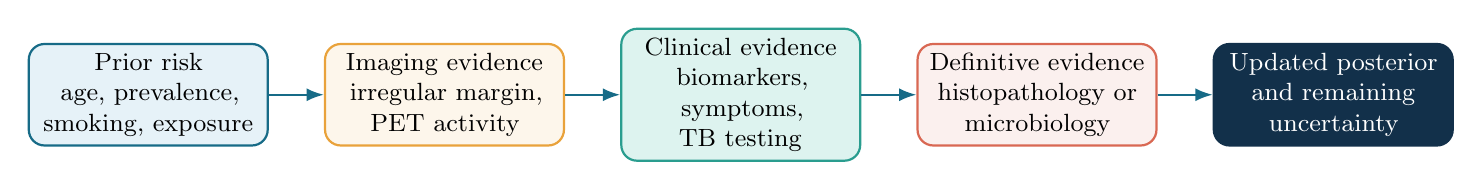
\begin{tikzpicture}[node distance=7mm]
  \node[box,text width=28mm] (prior) {Prior risk\\age, prevalence,\\smoking, exposure};
  \node[goldbox,right=of prior,text width=28mm] (img) {Imaging evidence\\irregular margin,\\PET activity};
  \node[tealbox,right=of img,text width=28mm] (lab) {Clinical evidence\\biomarkers, symptoms,\\TB testing};
  \node[coralbox,right=of lab,text width=28mm] (path) {Definitive evidence\\histopathology or\\microbiology};
  \node[darkbox,right=of path,text width=28mm] (post) {Updated posterior\\and remaining\\uncertainty};
  \draw[flow] (prior)--(img); \draw[flow] (img)--(lab); \draw[flow] (lab)--(path); \draw[flow] (path)--(post);
\end{tikzpicture}
\caption{Sequential Bayesian updating as new evidence becomes available.}
\end{figure}

\begin{keybox}
\textbf{Illustrative, not clinical probabilities:} an interface might display lung cancer 62\%, tuberculosis 27\%, and benign nodule 11\%. These numbers are useful only if calibrated on a relevant population and accompanied by uncertainty, provenance, and model limitations.
\end{keybox}

\section{Five Explainable AI Features}

\subsection{1. Patient-specific evidence ledger}
For every candidate diagnosis, show features that raise probability, features that lower it, missing evidence, and evidence quality. A doctor can distinguish ``the model saw this'' from ``this is generally associated with the disease.''

\subsection{2. Visual explanations for images}
Overlay lesion segmentation, measurements, comparison with prior scans, and carefully validated saliency. The interface must warn that a heat map shows model attention, not causal proof or pathology confirmation.

\subsection{3. Ranked differential with calibrated uncertainty}
Display multiple alternatives, credible or confidence intervals, calibration status, out-of-distribution warnings, and an abstention state. Include the next test expected to reduce uncertainty.

\subsection{4. Guideline, literature, data, and model provenance}
Link each recommendation to the exact guideline version, publication date, evidence passage, model version, data timestamp, and unavailable inputs. This forms a reproducible audit trail.

\subsection{5. Counterfactuals, override, and accountability}
Explain how plausible evidence changes would alter the ranking; allow doctors to override, record a reason, request multidisciplinary review, report bias, and attach the confirmed outcome. Preserve both the original output and the final human decision.

\begin{landscape}
\section{XAI Clinical Dashboard Concept}
\begin{figure}[H]
\centering
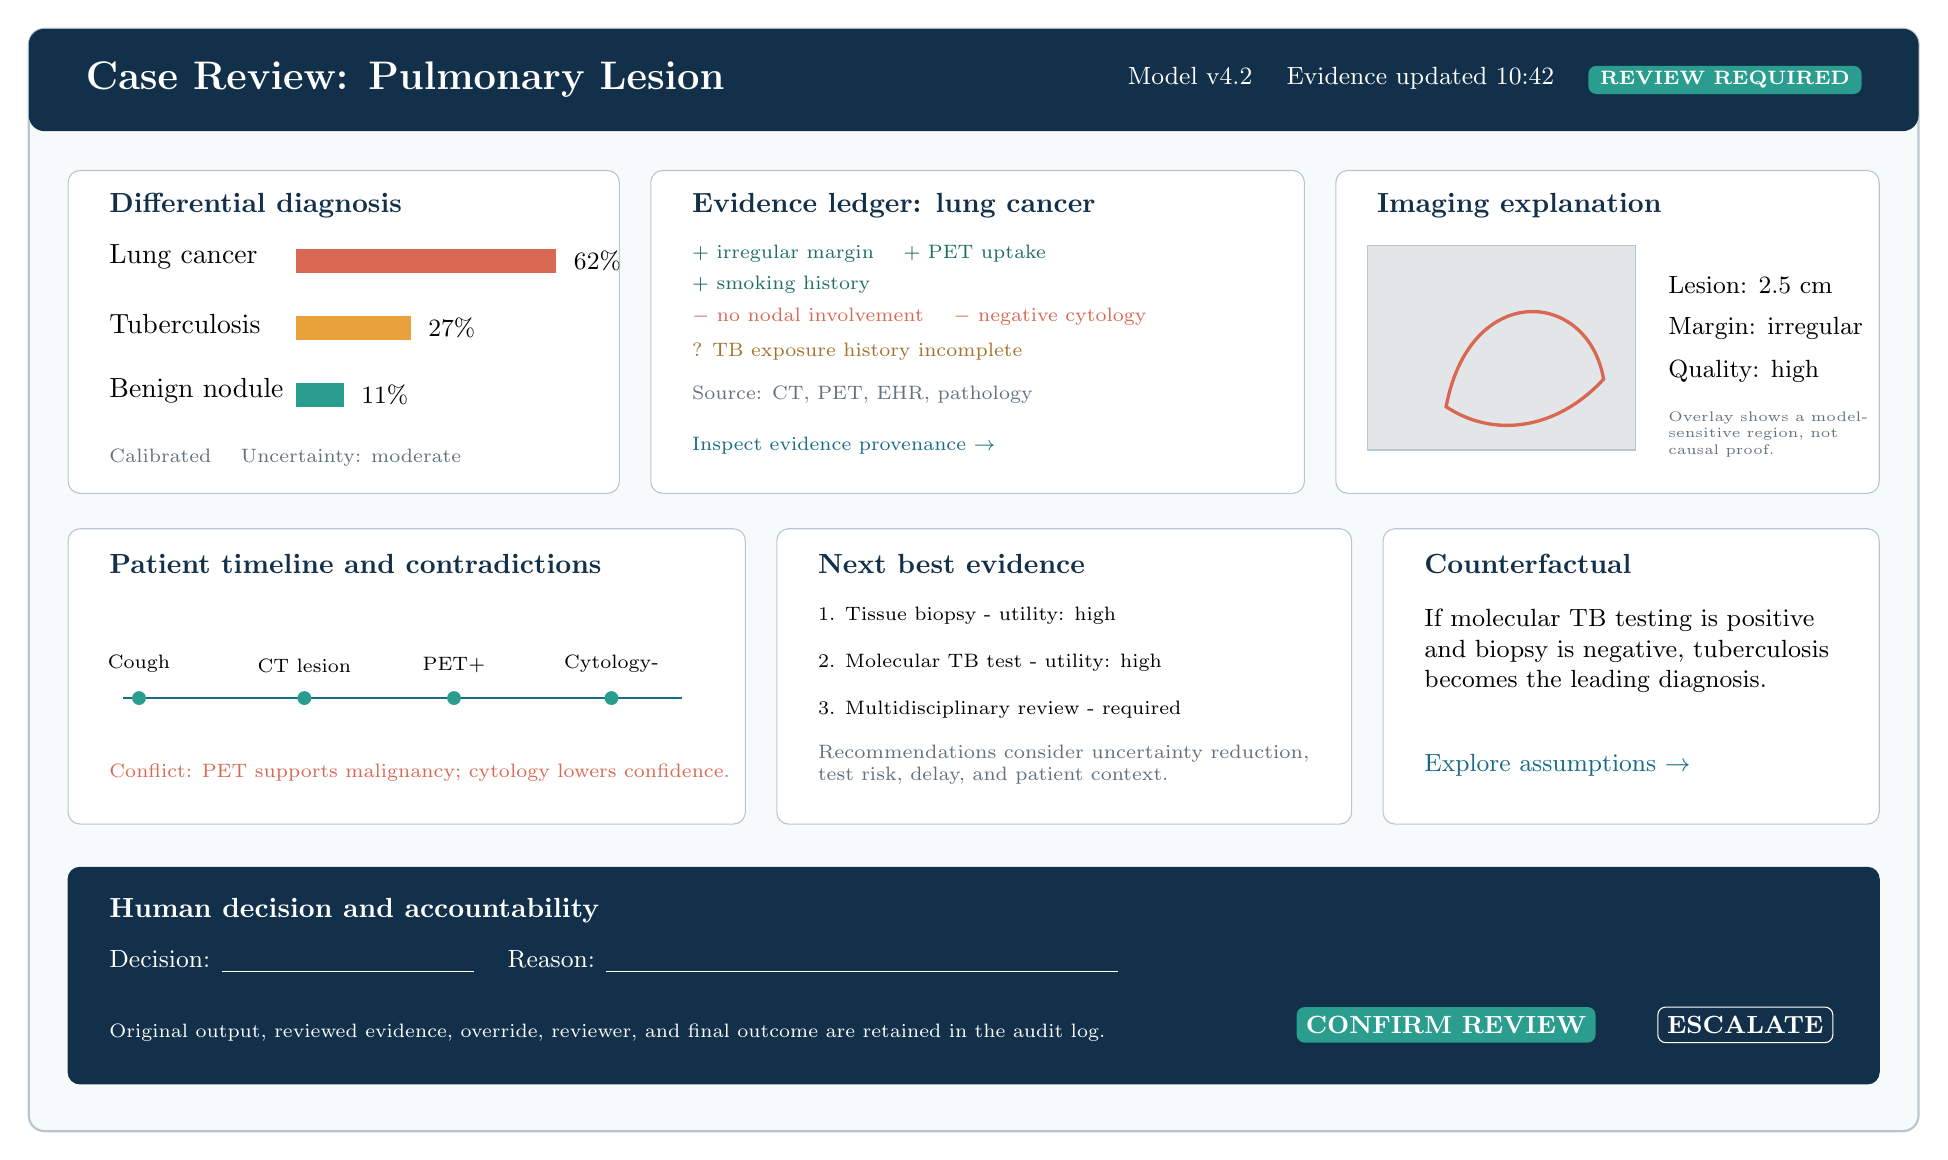
\begin{tikzpicture}[x=1cm,y=1cm]
  \draw[rounded corners=2mm,fill=paper,draw=line,thick] (0,0) rectangle (24,14);
  \fill[navy,rounded corners=2mm] (0,12.7) rectangle (24,14);
  \node[anchor=west,text=white,font=\Large\bfseries] at (.6,13.35) {Case Review: Pulmonary Lesion};
  \node[anchor=east,text=white,font=\small] at (23.4,13.35) {Model v4.2 \quad Evidence updated 10:42 \quad \badge{REVIEW REQUIRED}};

  \draw[rounded corners=1.5mm,fill=white,draw=line] (.5,8.1) rectangle (7.5,12.2);
  \node[anchor=west,font=\bfseries\color{navy}] at (.9,11.75) {Differential diagnosis};
  \node[anchor=west] at (.9,11.1) {Lung cancer}; \fill[coral] (3.4,10.9) rectangle (6.7,11.2); \node[anchor=west,font=\small] at (6.8,11.05) {62\%};
  \node[anchor=west] at (.9,10.25) {Tuberculosis}; \fill[gold] (3.4,10.05) rectangle (4.85,10.35); \node[anchor=west,font=\small] at (4.95,10.2) {27\%};
  \node[anchor=west] at (.9,9.4) {Benign nodule}; \fill[teal] (3.4,9.2) rectangle (4.0,9.5); \node[anchor=west,font=\small] at (4.1,9.35) {11\%};
  \node[anchor=west,font=\scriptsize\color{muted}] at (.9,8.55) {Calibrated \quad Uncertainty: moderate};

  \draw[rounded corners=1.5mm,fill=white,draw=line] (7.9,8.1) rectangle (16.2,12.2);
  \node[anchor=west,font=\bfseries\color{navy}] at (8.3,11.75) {Evidence ledger: lung cancer};
  \node[anchor=west,font=\scriptsize\color{teal!70!black}] at (8.3,11.15) {$+$ irregular margin \quad $+$ PET uptake};
  \node[anchor=west,font=\scriptsize\color{teal!70!black}] at (8.3,10.75) {$+$ smoking history};
  \node[anchor=west,font=\scriptsize\color{coral}] at (8.3,10.35) {$-$ no nodal involvement \quad $-$ negative cytology};
  \node[anchor=west,font=\scriptsize\color{gold!70!black}] at (8.3,9.9) {? TB exposure history incomplete};
  \node[anchor=west,font=\scriptsize\color{muted}] at (8.3,9.35) {Source: CT, PET, EHR, pathology};
  \node[anchor=west,font=\scriptsize\color{blue}] at (8.3,8.7) {Inspect evidence provenance $\rightarrow$};

  \draw[rounded corners=1.5mm,fill=white,draw=line] (16.6,8.1) rectangle (23.5,12.2);
  \node[anchor=west,font=\bfseries\color{navy}] at (17,11.75) {Imaging explanation};
  \draw[fill=navy!12,draw=line] (17,8.65) rectangle (20.4,11.25);
  \draw[coral,very thick] (18,9.2) .. controls (18.3,10.8) and (19.8,10.7) .. (20,9.55)
      .. controls (19.4,8.9) and (18.6,8.8) .. cycle;
  \node[anchor=west,font=\small] at (20.7,10.75) {Lesion: 2.5 cm};
  \node[anchor=west,font=\small] at (20.7,10.2) {Margin: irregular};
  \node[anchor=west,font=\small] at (20.7,9.65) {Quality: high};
  \node[anchor=west,font=\tiny\color{muted},text width=25mm] at (20.7,8.85) {Overlay shows a model-sensitive region, not causal proof.};

  \draw[rounded corners=1.5mm,fill=white,draw=line] (.5,3.9) rectangle (9.1,7.65);
  \node[anchor=west,font=\bfseries\color{navy}] at (.9,7.2) {Patient timeline and contradictions};
  \draw[thick,blue] (1.2,5.5)--(8.3,5.5);
  \foreach \x/\lab in {1.4/Cough,3.5/CT lesion,5.4/PET+,7.4/Cytology-}
    {\fill[teal] (\x,5.5) circle (2.5pt); \node[anchor=south,font=\scriptsize,align=center] at (\x,5.7) {\lab};}
  \node[anchor=west,font=\scriptsize\color{coral}] at (.9,4.55) {Conflict: PET supports malignancy; cytology lowers confidence.};

  \draw[rounded corners=1.5mm,fill=white,draw=line] (9.5,3.9) rectangle (16.8,7.65);
  \node[anchor=west,font=\bfseries\color{navy}] at (9.9,7.2) {Next best evidence};
  \node[anchor=west,font=\scriptsize] at (9.9,6.55) {1. Tissue biopsy - utility: high};
  \node[anchor=west,font=\scriptsize] at (9.9,5.95) {2. Molecular TB test - utility: high};
  \node[anchor=west,font=\scriptsize] at (9.9,5.35) {3. Multidisciplinary review - required};
  \node[anchor=west,font=\scriptsize\color{muted},text width=62mm] at (9.9,4.65) {Recommendations consider uncertainty reduction, test risk, delay, and patient context.};

  \draw[rounded corners=1.5mm,fill=white,draw=line] (17.2,3.9) rectangle (23.5,7.65);
  \node[anchor=west,font=\bfseries\color{navy}] at (17.6,7.2) {Counterfactual};
  \node[anchor=north west,font=\small,text width=52mm] at (17.6,6.75) {If molecular TB testing is positive and biopsy is negative, tuberculosis becomes the leading diagnosis.};
  \node[anchor=west,font=\small\color{blue}] at (17.6,4.65) {Explore assumptions $\rightarrow$};

  \draw[rounded corners=1.5mm,fill=navy,draw=navy] (.5,.6) rectangle (23.5,3.35);
  \node[anchor=west,text=white,font=\bfseries] at (.9,2.8) {Human decision and accountability};
  \node[anchor=west,text=white,font=\small] at (.9,2.15) {Decision: \underline{\hspace{32mm}} \quad Reason: \underline{\hspace{65mm}}};
  \node[rounded corners=1mm,fill=teal,text=white,font=\small\bfseries] at (18.0,1.35) {CONFIRM REVIEW};
  \node[rounded corners=1mm,draw=white,text=white,font=\small\bfseries] at (21.8,1.35) {ESCALATE};
  \node[anchor=west,text=white!70,font=\scriptsize] at (.9,1.25) {Original output, reviewed evidence, override, reviewer, and final outcome are retained in the audit log.};
\end{tikzpicture}
\caption{Conceptual dashboard showing the five XAI features as a single clinical workflow. Values are illustrative only.}
\end{figure}
\end{landscape}

\section{Continuous Learning, Governance, and Accountability}

Physician feedback is valuable only when linked to a reliable outcome and evaluated before deployment. Production models should be immutable during a case. New versions pass through offline curation, bias testing, clinical validation, approval, staged rollout, and monitoring.

\begin{figure}[ht]
\centering
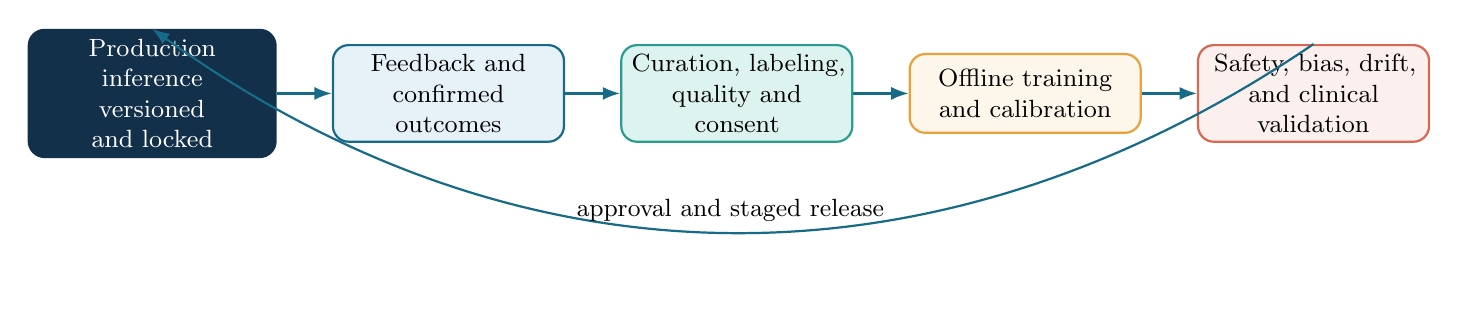
\begin{tikzpicture}[node distance=7mm]
  \node[darkbox,text width=29mm] (prod) {Production inference\\versioned and locked};
  \node[box,right=of prod,text width=27mm] (fb) {Feedback and\\confirmed outcomes};
  \node[tealbox,right=of fb,text width=27mm] (curate) {Curation, labeling,\\quality and consent};
  \node[goldbox,right=of curate,text width=27mm] (train) {Offline training\\and calibration};
  \node[coralbox,right=of train,text width=27mm] (validate) {Safety, bias, drift,\\and clinical validation};
  \draw[flow] (prod)--(fb); \draw[flow] (fb)--(curate); \draw[flow] (curate)--(train); \draw[flow] (train)--(validate);
  \draw[flow,bend left=35] (validate.north) to node[above,font=\small]{approval and staged release} (prod.north);
\end{tikzpicture}
\caption{Governed learning loop: feedback informs the next validated version, never an uncontrolled live mutation.}
\end{figure}

\subsection{Risk controls}
\begin{tabularx}{\textwidth}{>{\bfseries\color{blue}}p{31mm} X X}
\toprule
Concern & Design control & Evidence of accountability\\
\midrule
Bias & Subgroup performance, calibration, data-representation checks, fairness review, external validation & Versioned evaluation report and deployment gate\\
Transparency & Patient-level evidence, model card, guideline provenance, known limitations & Reproducible explanation bundle saved with case\\
False positive & Confirmation workflow, threshold tuning, uncertainty display, test-risk awareness & Sensitivity/specificity by use case and error review\\
False negative & High-sensitivity screening where appropriate, escalation triggers, abstention, post-market monitoring & Missed-case audit and safety incident process\\
Ethical responsibility & Meaningful human control, informed workflow, privacy, access controls, patient-centered tradeoffs & Named clinical reviewer and decision rationale\\
Legal accountability & Intended-use definition, audit logs, validation records, change control, retention policy & Trace from data and model version to recommendation and final action\\
\bottomrule
\end{tabularx}

\begin{figure}[ht]
\centering
\resizebox{\textwidth}{!}{%
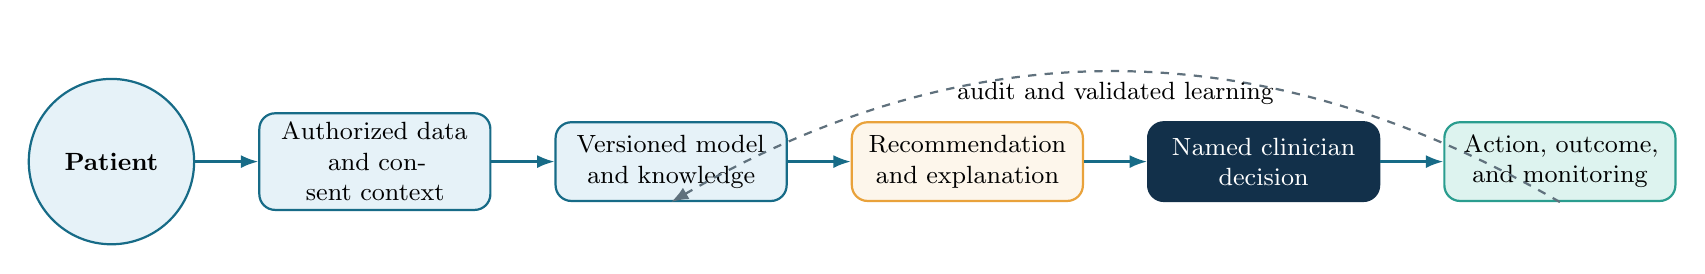
\begin{tikzpicture}[node distance=7mm and 8mm]
  \node[circlebox,minimum size=21mm] (patient) {Patient};
  \node[box,right=of patient,text width=27mm] (data) {Authorized data\\and consent context};
  \node[box,right=of data,text width=27mm] (model) {Versioned model\\and knowledge};
  \node[goldbox,right=of model,text width=27mm] (rec) {Recommendation\\and explanation};
  \node[darkbox,right=of rec,text width=27mm] (doc) {Named clinician\\decision};
  \node[tealbox,right=of doc,text width=27mm] (outcome) {Action, outcome,\\and monitoring};
  \draw[flow] (patient)--(data); \draw[flow] (data)--(model); \draw[flow] (model)--(rec); \draw[flow] (rec)--(doc); \draw[flow] (doc)--(outcome);
  \draw[softflow,bend right=30] (outcome.south) to node[below,font=\small]{audit and validated learning} (model.south);
\end{tikzpicture}}
\caption{Accountability chain from patient context to monitored outcome.}
\end{figure}

\section{Recommended Operating Workflow}

\begin{enumerate}[label=\protect\badge{\arabic*},leftmargin=11mm,itemsep=4pt]
  \item Verify identity, permissions, data freshness, modality quality, and missing inputs.
  \item Run modality-specific models and preserve their independent outputs.
  \item Fuse evidence, retrieve applicable knowledge, and compute a calibrated differential.
  \item Trigger deliberate review for disagreement, low confidence, rare cases, distribution shift, or high-consequence decisions.
  \item Present evidence, uncertainty, provenance, counterfactuals, and next-test utility.
  \item Require clinician review; record acceptance, modification, override, or escalation.
  \item Link confirmed outcomes to the case and monitor errors, drift, and subgroup performance.
  \item Retrain only through the governed validation and approval pipeline.
\end{enumerate}

\section{Conclusion}

The proposed cognitive system combines NLP, machine learning, deep learning, a curated knowledge base, probabilistic reasoning, XAI, and visualization into one human-governed clinical workflow. System 1 supplies rapid pattern recognition and hypothesis generation; System 2 challenges those hypotheses, integrates contradictory evidence, and seeks the most informative next step.

Probabilistic reasoning is better suited than rigid rules because cancer diagnosis is inherently uncertain and multimodal. Trust comes not from a persuasive score, but from calibrated performance, visible limitations, traceable evidence, meaningful physician control, and a complete accountability chain.

\begin{keybox}
\centering
\Large\bfseries\color{navy}
AI proposes and explains. Clinicians interrogate and decide. Governance makes both accountable.
\end{keybox}

\section*{Selected References}
\addcontentsline{toc}{section}{Selected References}
\begin{enumerate}[label={[\arabic*]},leftmargin=8mm]
  \item D. Kahneman, \emph{Thinking, Fast and Slow}. Farrar, Straus and Giroux, 2011.
  \item World Health Organization, \emph{Ethics and Governance of Artificial Intelligence for Health}, 2021.
  \item U.S. National Institute of Standards and Technology, \emph{Artificial Intelligence Risk Management Framework (AI RMF 1.0)}, 2023.
  \item A. B. Arrieta et al., ``Explainable Artificial Intelligence (XAI): Concepts, taxonomies, opportunities and challenges toward responsible AI,'' \emph{Information Fusion}, vol. 58, 2020.
\end{enumerate}

\end{document}
